% Project final report length limit: 10 pages, single-column standard latex.
% Due date May 13. This is a strict deadline as we need to finish grading by the final grades
% due date. Final project and poster presentation account for 40% of the the grade.
% Pre-proposal accounted for 1% of grade.
\documentclass[a4paper, 10pt]{article}

\usepackage{caption}
\usepackage{float}
\usepackage{hyperref}
\hypersetup{
    colorlinks=true,
    linkcolor=blue,
    filecolor=magenta,      
    urlcolor=cyan,
    pdftitle={Overleaf Example},
    pdfpagemode=FullScreen,
}

\urlstyle{same}

\usepackage{xcolor}
\usepackage{graphicx}
\graphicspath{ {./images/} }

\definecolor{commentgreen}{RGB}{2,112,10}
\definecolor{eminence}{RGB}{108,48,130}
\definecolor{weborange}{RGB}{255,165,0}
\definecolor{frenchplum}{RGB}{129,20,83}
\usepackage{listings}
\lstset {
    language=C++,
    frame=tb,
    tabsize=4,
    showstringspaces=false,
    numbers=left,
    %upquote=true,
    commentstyle=\color{commentgreen},
    keywordstyle=\color{eminence},
    stringstyle=\color{red},
    basicstyle=\small\ttfamily, % basic font setting
    emph={int,char,double,float,unsigned,void,bool},
    emphstyle={\color{blue}},
    escapechar=\&,
    % keyword highlighting
    classoffset=1, % starting new class
    otherkeywords={>,<,.,;,-,!,=,~},
    morekeywords={>,<,.,;,-,!,=,~},
    keywordstyle=\color{weborange},
    classoffset=0,
}

% We can define some other document properties too!
\author{Rashad Gover}
\date{\today}
\title{Exploring Parallel Programming in Haskell}

\begin{document}

\maketitle

\newpage
\tableofcontents

\newpage

\begin{abstract}
  In this report, we will explore parallel computation in the pure functional language \textbf{\textit{Haskell}}.
\end{abstract}

\section{Brief Introduction to Haskell}
Haskell is a declarative, functional programming language invented in 1987 by a group of programming language researchers for the purpose of exploring the design space of functional languages. Unlike imperative languages which are based on turing machines and embrace state, Haskell and other pure functional languages are based on the lambda calculus, invented by Turing's professor Alonzo Church, where state is dropped in favor of mathematical functions. At a high-level, a Haskell program is just a function that is composed of many smaller functions. On top of being a functional programming language, Haskell is also a strongly, statically typed language which eliminates an entire class of errors (type errors) at compile-time. 

Haskell has all the basic features that you would expect from any programming language like variables, function declaration,  and a module system for decoupling code. Haskell also has more interesting features like type inferenece, user defined types, pattern matching, type classes, lazy evaluation by default, and monads for modelling side-effects without compromising purity. These traits, besides laziness, make Haskell a good candidate for implementing parallel algorithms. The declarative nature of Haskell allows the user to focus on the problem at hand instead of the low-level details such as state, the order in which statements are declared, and memory management.  Much of the burden that is usually placed on the shoulders of the programmer is pushed to the advanced compiler, which makes Haskell more "ergonomic" in my opinion. To show this, let's implement a program in C++ and Haskell that takes in an array or list, repspectively, and increments each value, doubles it, and then prints the values. The implementation in C++ would look something like this:

\begin{lstlisting}[language=C++, caption=C++ example]
#include <iostream>
int main() {
  int arrLength = 5;
  int arr [] = {1, 2, 3, 4, 5};
  for (int i = 0; i < arrLength; i++) {
    arr[i] += 1;
    arr[i] *= 2;
    std::cout << arr[i] << " ";
  }
  return 0;
}
\end{lstlisting}

The Haskell implementation would look like so:

\begin{lstlisting}[language=Haskell, caption=Haskell example]
module Main where
list = [1, 2, 3, 4, 5]
incThenDouble x = (x + 1) * 2
answer = map incThenDouble list
main = print answer
\end{lstlisting}

As we can see, the Haskell implementation is much more concise than the C++ implementation. You may also notice that compared to the Haskell version, the C++ version looks much like a "recipe" where each step of transforming the array in to another must be described in detail: how long the array is, how to loop through the array, the types of the variables, etc. The Haskell version on the other hand is very declarative, and as a result looks a lot cleaner and readable. Obviously, this is a contrived example, but in my experience it seems to be the case more often than not that Haskell code looks more approachable compared to an imperative language. The idea is that this same conciseness will carry over to parallel programs.

\subsection{Fibonacci Sequence}
The Fibonacci sequence is a series of numbers where a number is the addition of the last two numbers, starting with 0, and 1. The serial implementation in Haskell is very straightforward. The following isn't the fastest implementation, but is probably the most idiomatic:

\begin{lstlisting}[language=Haskell, caption=Haskell Fibonacci]
module SerialFib where

nfib :: Int -> Int
nfib 0 = 0
nfib 1 = 1
nfib n = nfib (n-1) + nfib (n-2)
\end{lstlisting}

We pattern match on the value of the integer: if the value is 0 return 0, and if it is 1 return 1. Otherwise, return the sum of fib of the previous fibonacci number and the fibonacci number before the previous one. 

The use of recursion has some performance implications. The memory performance of recursive functions in Haskell differs depending on whether or not the recursive function is \textbf{\textit{tail recursive}}. A recursive function is tail recursive if the final result of the recursive call is the final result of the function itself. If the result of the recursive call must be further processed, it is not tail recursive. So in the case above, the function \lstinline{nfib} is not tail recursive.

\subsection{Matrix Multiplication}

To represent matrix multiplication in Haskell, we use the \lstinline{Vector} data type over the more idiomatic \lstinline{List} data type. This is to enhance the performance of the serial program since \lstinline{List} in Haskel is a lazy data structure,  while a \lstinline{Vector} value represents an \textbf{\textit{unboxed array}} under the hood and thus has an \textit{O(1)} length operation and data access.

\begin{lstlisting}[language=Haskell, caption=Haskell MatMul]
module SerialMatMul where

import Data.Vector (Vector(..), (!))
import qualified Data.Vector as Vector

matMul
  :: (Eq a, Num a)
  => Vector (Vector a)
  -> Vector (Vector a)
  -> Either String (Vector (Vector a))
matMul a b
  | Vector.length a == 0 || Vector.length b == 0 = Left "Empty matrices can't be used"
  | not (isConsistentMatrix a) || not (isConsistentMatrix b) = Left "The dimensions of the matrices are inconsistent"
  | numOfCol a /= numOfRow b = Left "These matrices are incompatible for multiplication"
  | otherwise = Right $ mul a b
  where
    numOfCol m = Vector.length $ Vector.head m
    numOfRow m = Vector.length m
\end{lstlisting}

Ideally, to leverage the advanced type sytem of Haskell we would encode the length of the vectors in their types. The compiler would then be able to automatically handle any cases in which the dimensions of the matrices represented as vectors don't match up correctly. This is known as \textbf{\textit{type-level programming}} and it allows the programmer to encode information in types to provide more information for the compiler and further constrain the number of unwanted outcomes. I opted for the above implementation due to ease of implementation and better performance, but needed to add guards to check the dimensions of the matrices at the value-level.

\subsection{Benchmarking}

All benchmarks were recorded on my personal laptop. The machine used for all tests has 4 cores and 16GB RAM. I'm using some simple timer functions to get the times for my data, so they may not be the most accurate results:

\begin{lstlisting}[language=Haskell, caption=Clock functions]
currentTime = getCurrentTime

timeElapsedSince t0 = do
  t1 <- getCurrentTime
  printf "time: %.2fs\n" (realToFrac (diffUTCTime t1 t0) :: Double)
\end{lstlisting}

The results for the serial version of Fibonacci were interesting:

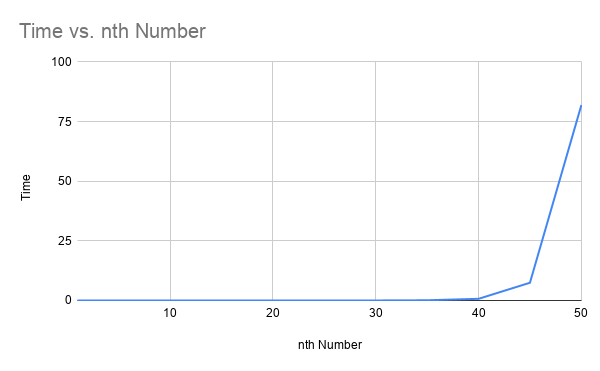
\includegraphics[scale=0.5]{serialFibData}

The function was able to able to handle calculating the Fibonacci numbers in a reasonable amount of time up until I tried to ask it for the 40th Fibonacci number and beyond. After asking for the 45th number, the time it took to come up with an answer increased exponentially. Asking for the 50th Fibonacci number took 81.94 seconds!

\section{Parallel Haskell}

There are various ways of expressing parallelism in Haskell ranging from monad-based libraries like \lstinline{monad-par} to embedded DSLs (Domain Specific Languages) like \lstinline{accelerate}. These libraries can be vastly different from one another, so the programmer must know how to choose the right tool for the job. Certain libraries will only really make sense for certain types of problems. To test these various methods of expressing parallelism, I've created a series of microbenchmarks to test them and compare them will serial versions of the same program.

\subsection{Dataflow Parallelism with monad-par}

Dataflow parallelism is best used for implementing parallel algorithms where the problem can be broken down into smaller pieces and solved recursively. Problems that would fit in this category are generating the nth Fibonacci number, mergesort, or traversing a binary tree. The best library I found for expressing dataflow parallelism is \lstinline{monad-par}. Monads are a \textit{class of types} that are commonly used in Haskell as a way to model functions that produce effects. Monads can express many different types of effects, such as non-determinism, state, IO with the outside world, and also parallelism. With out monads, these sort of effectful functions couldn't exist in a pure functional language like Haskell. The \lstinline{monad-par} library defines a monad for the user through which they can express parallel computation.

\subsubsection{Fibonacci Implementation}

Since \lstinline{monad-par} is great for problems that can be recursively broken down and solved, it is  a perfect fit for parallelizing the \lstinline{nfib} function defined earlier:

\begin{lstlisting}[language=Haskell, caption=Fibonnaci using monad-par library]
module MonadParFib where

import Control.Monad.Par

nfib :: Int -> Par Int
nfib n = do
  firstComputation <- spawn (nfib (n - 1))
  secondValue <- nfib (n - 2)
  firstValue <- get firstComputation
  return (firstValue + secondValue)
\end{lstlisting}

The \lstinline{spawn} function forks a new thread where the calculation of the previous Fibonacci number happens. Then,  the result of a second call to \lstinline{nfib} is produced. While the second value is being calculated, the first computation is still running or maybe already done. Once the second value has been produced, the value of the first computation must be extracted to use it. Finally, the two results are combined to produce the final answer. It helps to think of it as branching tree, where each call to \lstinline{nfib} produces two more branches that run in parallel.

It also important to note that the runtime of the `Par` monad is based on \textit{sparks} which are different than threads in the context of Haskell, where "threads" usually refer to green threads.

\subsubsection{Results}

Unfortunately, I was unable to obtain any useful results from benchmarking this function. My computer crashed even when asking for the 1st Fibonacci number, so it did really bad compared to the serial version, which is not what I expected. Trying to run the program on any amount of cores, from 1 - 4, produced no results. Each time the program ended with \lstinline{Killed} as the output. As far as I know, this means that the runtime ran out of memory or got hung up at a certain point in the program. I honestly don't know what went wrong here. My theory is that my machine is too weak, or the overhead of using \lstinline{monad-par} is too much. From my research, similar examples with branching logic seemed to work fine, so I'm not sure if it just has to do with my machine. Since the Haskell runtime is really complex, it's more likely that I missed an opportunity to make some part of the program strict instead of lazy, which Haskell is by default. I've been burned in the past by Haskell's laziness, so this wouldn't be the first time.

\subsection{Regular Parallel Arrays}

In contrast to dataflow parallelism which is great for recursive problems, Haskell has an array-based library called \lstinline{repa} that is great for any problems that can be modelled as an array. \lstinline{repa} gives you the ability to represent polymorphic, parallel arrays in Haskell, which is a big step up from the more commonly used, but less performant \lstinline{List} or \lstinline{Vector} data types. Any functions that use the data structures and special operators provided by the  \lstinline{repa} library are automatically parallelized by simply passing in a flag to GHC (Glasgow Haskell Compiler). This makes it easy to parallelize serial code that use sequential data structures ineffeciently.

\subsubsection{Matrix Multiplication Implementation}

The \lstinline{repa} library is an obvious fit for parallelizing matrix multiplication. Instead of using a nested \lstinline{Vector} data type to represent a matrix, we can use the array shapes provided by the `repa` library:

\begin{lstlisting}[language=Haskell, caption=Matrix multiplication using repa library]
module RepaMatMul where

import Data.Array.Repa (Array(..), U(..), Z(..), DIM2(..), (:.)(..))
import Data.Array.Repa as Repa
import Data.Vector.Unboxed.Base (Unbox(..))

matMul
  :: (Monad m, Num a, Unbox a)
  => Array U DIM2 a
  -> Array U DIM2 a
  -> m (Array U DIM2 a)
matMul a b = Repa.sumP (Repa.zipWith (*) aNew bNew)
    where
      bTranspose = Repa.transpose b
      (Z :. aCols :. aRows) = Repa.extent a
      (Z :. bCols :. bRows) = Repa.extent b
      aNew = Repa.extend (Z :. All :. bCols :. All) a
      bNew = Repa.extend (Z :. aRows :. All :. All) bTranspose
\end{lstlisting}

The nice thing about this implementation is that not only is it more performant that the serial implementation introduced earlier, but it also more \textit{type safe}, meaning that the compiler can better catch our mistakes because it knows more about the program at compile-time. If you look at the type signature of the \lstinline{matMul} function, you can see that it provides the shape of the array and the exact dimensions of the array. In our case, we are using an array of 2 dimensions, so the \lstinline{Array} type is given the type \lstinline{DIM2} as an argument to represent this. These more detailed types also allow the Haskell runtime to make better optimizations to the code.

\subsubsection{Results}

I also failed to obtain any useful results from benchmarking this function either, which is a shame because I spent a lot of time implementing this one. My theory is that I was unable to effeciently convert from the \lstinline{List} data type to the \lstinline{repa} data types that are required for the parallelism to work. After discussion with community memebers, it seems that the function should work correctly, but the IO that I perform to setup the function for testing maybe the bottleneck.

\subsection{Particle Simulation with Accelerate Library}

Implementing a particle simulator in Haskell using the \lstinline{accelerate} library was the main focus of the paper, but like my \lstinline{monad-par} and \lstinline{repa} implementations, I was unable to obtain any meaningful results. I reached out to the official maintainer of the library to see what I could do, but received no response. The community reccomended that I use another similar library called \lstinline{massiv} to see what happens. I was too deep in and decided to go forward with what I had, but ultimately came to no conclusion on whether or not \lstinline{accelerate} is effective for particle simulation. I was inspired by the examples provided by the \lstinline{accelerate} library and everything type-checked and compiled, but was I unable to benchmark the simulation function and get useful results.

\section{Honorable Mentions}

There were some other paths that I went down on my journey to proving Haskell useful in a parallel computing context. Besides the  \lstinline{monad-par} library, there is a similar library called \lstinline{strategies} that cought my eye early on, but I dropped it due to its' similarity to \lstinline{monad-par}. Now I wonder if going with \lstinline{strategies} would've produced a better outcome, but I can't be sure.

Another worthy mention are a group of functions I implemented for microbenchmarking called \lstinline{checkAll} (serial) and \lstinline{checkAllPar} (parallel) which check to see if every value in a binary tree satisfy a given predicate. I used the \lstinline{monad-par} library to implement this due to its' branching, recursive nature and ran into the same issues I ran into with my implementation of the Fibonnaci sequence solver. Since it is nearly identical to my Fibonacci example, I left it out to pursue the more interesting aspects of the project, but feel free to check out the repository code if you're interested in seeing how it works. Here's what the code for those functions looks like:

\begin{lstlisting}[language=Haskell, caption=Serial Tree check]
module Tree.SerialTree where

data Tree a = Leaf a
            | Node (Tree a) (Tree a)
  deriving (Eq, Show)

-- Check that all values in the tree satisfy a given predicate
checkAll :: (a -> Bool) -> Tree a -> Bool
checkAll pred (Leaf value) = pred value
checkAll pred (Node leftTree rightTree) = (checkAll pred leftTree) && (checkAll pred rightTree)
\end{lstlisting}

\begin{lstlisting}[language=Haskell, caption=Tree check using monad-par]
module Tree.MonadParTree where

import Tree.SerialTree (Tree(..))
import Control.Monad.Par

-- Test whether all elements match the given predicate (in parallel)
checkAllPar :: (a -> Bool) -> Tree a -> Par Bool
checkAllPar pred (Leaf value) = return $ pred value
checkAllPar pred (Node leftTree rightTree) = do
  leftTreeComputation <- spawn $ checkAllPar pred leftTree
  rightTreeResult  <- checkAllPar pred rightTree
  leftTreeResult  <- get leftTreeComputation
  return $ leftTreeResult && rightTreeResult
\end{lstlisting}

\section{Conclusion}

All in all, I can truly say that my initial hypothesis of Haskell being a more "ergonomic" language than a traditional imperative language for expressing parallel algorithms was wrong. Yes, the code may be more concise and prettier, but the setup and tooling around parallel programming seems to be lacking when compared to other languages. I found little resources and knowledge on benchmarking and reasoning about parallelism in Haskell. As a Haskell developer of a couple years now, even reasoning about serial code can be difficult, but I didn't expect parallelism in Haskell to be this much harder. 

Another pain point I experienced was laziness. Laziness makes predicting what the runtime is going to do a lot more difficult and it really hurt me. In the back of my head, I still wonder if some of my benchmarks weren't working simply because of a failure to reduce a thunk or use a strict data type. Laziness does provide by benefits, like forcing the language to be pure and having the ability to produce streams of data easily, but for parallel programming lazy evaluation is definitely a pain.

Last but not least, I failed on my part to find a strong machine to test my programs out on. I was unable to setup the Haskell environment on CORI, so my laptop was the best option knowing what I knew at the time I started this project. If I could do it over again, I would use a machine on Digital Ocean or AWS to rule out any sort of issues that may have been caused by using a machine that is too weak.

The best things about the project were that I got to get more familiar with one of my favorite programming languages, and got to see parallel programming from another perspective that it isn't seen from often.
So to answer to the question I initially had at the start of this journey, I would say that Haskell is most definitely not the best tool for parallel programming. I wasn't expecting it to be, but at the same time, I didn't expect the experience to be as bad as it was. At the end of the day, I must also consider my lack of skill and the fact that I wasn't able to devote 100\% of my focus to this project as I would've liked. I hope one day I can revisit this project and give it the conclusion it deserves.


\section{Prior Work \& Resources}

\begin{enumerate}
	\item GitHub repo for the entire project: \url{https://github.com/rashadg1030/cs267-final}
	\item Reference for GHC (Glasgow Haskell Compiler): \url{https://www.haskell.org/ghc/}
	\item Book by Simon Marlow on Parallel and Concurrent Programming in Haskell: \url{https://www.oreilly.com/library/view/parallel-and-concurrent/9781449335939/}
	\item Documentation for \lstinline{monad-par} library: \url{http://hackage.haskell.org/package/monad-par}
	\item A blog post on using the \lstinline{monad-par} library: \url{http://tomasp.net/blog/speculative-par-monad.aspx/}
	\item Documentation for \lstinline{repa} library: \url{https://hackage.haskell.org/package/repa-3.4.1.4/docs/Data-Array-Repa.html}
	\item A tutorial for using \lstinline{repa}: \url{https://wiki.haskell.org/Numeric_Haskell:_A_Repa_Tutorial}
	\item Documentation for \lstinline{accelerate} library: \url{https://hackage.haskell.org/package/accelerate-1.3.0.0/docs/Data-Array-Accelerate.html}
	\item A compilation of examples of \lstinline{accelerate} in use: \url{https://github.com/AccelerateHS/accelerate-examples}
	\item An academic paper on parallel evaluation strategies in Haskell: \url{http://simonmar.github.io/bib/papers/strategies.pdf}
	\item Great resource for learning LaTeX: \url{https://www.overleaf.com/}
\end{enumerate}

\end{document}